\chapter{Experimental evaluation}
\label{ch:experiments}

``In this chapter, we present experimental results on the algorithms proposed and we compare them with state of the art methods." 

\section{Experimental setting}

\begin{table}[ht]
\centering
\renewcommand{\arraystretch}{1.2}
\begin{tabular}{|l|c|c|c|c|c|}\hline
\textbf{Name}&$n$&$m$&Average degree&Max $In(v)$&Max $Out(v)$\\ \hline\hline
Email&971&3466&3.57&4&47\\ \hline
\end{tabular}
\caption{Dataset used for the experiment.}
\label{tb:elf_datasets}
\end{table}

\paragraph{Datasets} \autoref{tb:elf_datasets} shows the characteristics of the dataset used for the experiment. The dataset is a subgraph obtained from a real dataset provided by SNAP \cite{snapnets}, \emph{email-Eu-core}, generated using email data from a large European research institution. A directed edge $(u, v)$ means that person $u$ sent an e-mail to person $v$.

As widely done in literature, we assigned the ground-truth influence probabilities according to the weighted cascade model, that is, $p_{u,v}=\frac{1}{|In(v)|}$, for each edge $(u,v) \in E$.

\paragraph{Algorithms}

For the learning process, we use the Thompson Sampling (TS) as principal exploration strategy (\autoref{alg:cts}). For the sake of completeness, we show also results with a Pure Exploitation (PE) approach, in which the oracle is fed with the mean estimates of the influence probabilities at each round.

\section{Results}

\paragraph{Experiment 1}
In this experiment, we test the algorithms on Email over a time horizon of $T=100$ rounds. The objective is to show the performances of the algorithms. The results have been averaged over 30 runs. \autoref{fig:exp_email} shows the cumulative regret, with a 95\% confidence interval.

\begin{figure}[H]
  \centering
  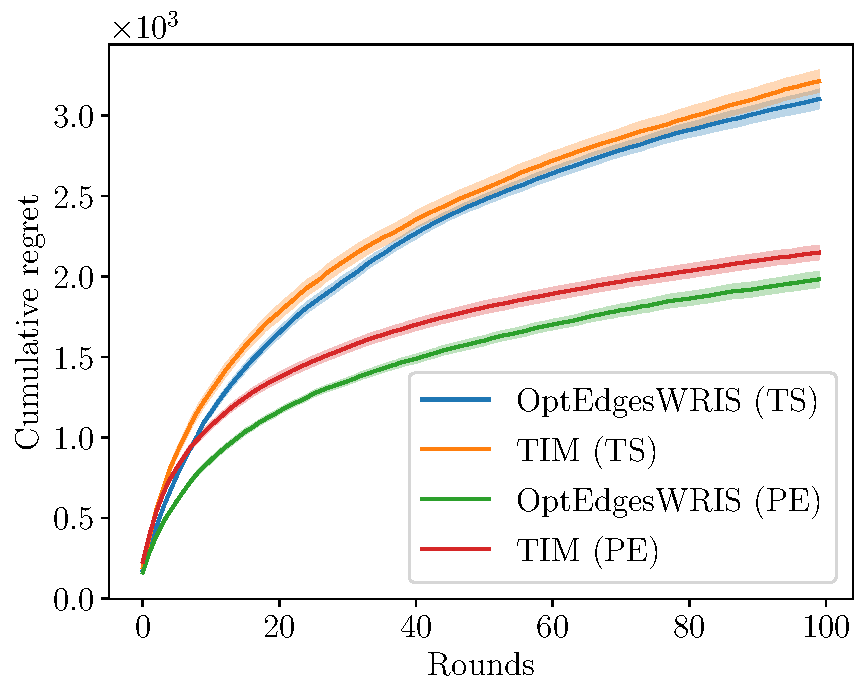
\includegraphics[width=.65\textwidth]{experiments/regret.pdf}
\caption{Cumulative regret in Email-In4 with 95\% confidence interval.}
\label{fig:exp_email}
\end{figure}

As shown in the plot, our algorithm performs better with both the exploration strategies. However, the gain on TIM is more evident with the PE strategy, specially in the first rounds.